\documentclass{beamer}


\usetheme{CambridgeUS}
%\usetheme{Singapore}
\usefonttheme[onlylarge]{structurebold}
\setbeamerfont*{frametitle}{size=\normalsize,series=\bfseries}
\setbeamertemplate{navigation symbols}{}
\setbeamertemplate{headline}


%\usefoottemplate{%
%\tinycolouredline{structure}%
%{\color{white}\textbf{Company Name\hfill Company Proprietary}}%
%}

\setbeamertemplate{footline} {%
  \hbox{%
  \begin{beamercolorbox}[wd=.20\paperwidth,ht=2.25ex,dp=1ex,center]{author in head/foot}%
    \usebeamerfont{author in head/foot}\insertshortinstitute, \the \year
  \end{beamercolorbox}%
  \begin{beamercolorbox}[wd=.70\paperwidth,ht=2.25ex,dp=1ex,center]{title in head/foot}%
    \usebeamerfont{title in head/foot}\insertshorttitle
  \end{beamercolorbox}%
  \begin{beamercolorbox}[wd=.10\paperwidth,ht=2.25ex,dp=1ex,right]{date in head/foot}%
    \usebeamerfont{date in head/foot}
    \insertframenumber{} / \inserttotalframenumber\hspace*{2ex} 
  \end{beamercolorbox}
  }
}



\setbeamercolor*{author in head/foot}{parent=palette tertiary}
\setbeamercolor*{title in head/foot}{parent=palette secondary}
\setbeamercolor*{date in head/foot}{parent=palette primary}


% Standard packages
%\usepackage[brazil]{babel}
\usepackage{latexsym}
\usepackage{verbatim}
\usepackage{comment}
\usepackage[T1]{fontenc}
\usepackage{datetime}
\usepackage{listings}
\usepackage{color}

\definecolor{orange}{rgb}{1,0.5,0}

	%fontes:
%\usepackage{tgschola}
%\usepackage{venturisold}
\usepackage{bookman}
\usepackage{datetime}
%\usepackage{mathptmx}
%\usepackage{times}
%\usepackage{lmodern}
%\usepackage{fourier}
%\usepackage[scaled]{berasans}
%\usepackage[default]{gfsbodoni}
%\renewcommand*\familydefault{\sfdefault}  %% Only if the base font of the document is to be sans serif


\usepackage[latin1]{inputenc} %para utilizar acentos

%\usepackage[dvips]{graphicx}



\usepackage{tikz}
\usetikzlibrary{arrows}
\tikzstyle{block}=[draw opacity=0.7,line width=1.4cm]



\newcommand{\aspas}[1]{{``#1''}}

\newcommand{\aspassimples}[1]{{`#1'}}

\newcommand{\variavel}[1]{{\texttt{\textbf{#1}}}}
\newcommand{\var}[1]{{\texttt{\textbf{#1}}}}

\newcommand{\variaveldestaque}[1]{{\textcolor{blue}{\texttt{\textbf{#1}}}}}


% The main document

\begin{document}

\lstset{language=C,
        format=C,
        numbers=left,
        numberstyle=\Tiny, 
        stepnumber=2,
        numberfirstline=auto,
        firstnumber=auto,
        numbersep=5pt,
        captionpos=b,
        xleftmargin=0.3cm,
        xrightmargin=0cm,
        framexbottommargin=0cm,
        framextopmargin=0cm,
        tabsize=4,
        boxpos=c,
        frame=no,
        basicstyle=\scriptsize,
        commentstyle=\it\color{gray},
        showstringspaces=false
}

\let\olditemize=\itemize
\let\endolditemize=\enditemize
\renewenvironment{itemize}{%
    \begin{olditemize}%
      \setlength{\itemsep}{0.3cm}%
  }%
  {%
    \end{olditemize}%
  }
  
  \newenvironment{itemize2}{%
    \begin{olditemize}%
      \setlength{\itemsep}{0.2cm}%
  }%
  {%
    \end{olditemize}%
  }

\AtBeginSection % Do nothing for \section* 
{ 
\begin{frame}{}
\frametitle{} 
%\tableofcontents[currentsection,subsectionstyle=show/show/hide,square]
\begin{block}

\centering{\usebeamerfont{title}\usebeamercolor[fg]{title}\insertsectionhead}
\end{block}

\end{frame} 
}


%\setbeamertemplate{title page}
{

\begin{figure}
     
\includegraphics[width=1.8cm]{ufmg.png}
     \hspace{230pt}
     
\includegraphics[width=1.8cm]{ppgcc.png}
\end{figure}


\begin{block}

\centering{\usebeamerfont{title}\usebeamercolor[fg]{title}\inserttitle}
\end{block}

\vspace{30pt}

\begin{table}[htdp]
\begin{center}
\begin{tabular}{cp{2cm}c}
Ricardo Terra\\
{\scriptsize terra@dcc.ufmg.br}
\end{tabular}
\end{center}
\end{table}%


\vspace{40pt}
\begin{beamercolorbox}[center,shadow=false]{}
\small \today
\end{beamercolorbox}

\vspace{40pt}
}

\begin{frame}
  \titlepage
\end{frame} %Abre documento

\title[Setting up $\bf dclsuite$] 
{%
  Setting up $\bf dclsuite$%
}

\author[Evento (rodapé)]
{%
  Evento%
}

\institute[DCL]
{%
DCL%
}

%\date[\monthname,  \the \year, \today ]
\date[Mês, Ano]


\setbeamertemplate{title page}
{

\begin{figure}
     
\includegraphics[width=1.8cm]{ufmg.png}
     \hspace{230pt}
     
\includegraphics[width=1.8cm]{ppgcc.png}
\end{figure}


\begin{block}

\centering{\usebeamerfont{title}\usebeamercolor[fg]{title}\inserttitle}
\end{block}

\vspace{30pt}

\begin{table}[htdp]
\begin{center}
\begin{tabular}{cp{2cm}c}
Ricardo Terra\\
{\scriptsize terra@dcc.ufmg.br}
\end{tabular}
\end{center}
\end{table}%


\vspace{40pt}
\begin{beamercolorbox}[center,shadow=false]{}
\small \today
\end{beamercolorbox}

\vspace{40pt}
}

\begin{frame}
  \titlepage
\end{frame} %Insere capa


\begin{frame}{\inserttitle}
	\begin{block}{\tiny Extract the contents of $\tt dclsuite.zip$ into Eclipse directory}
		\centering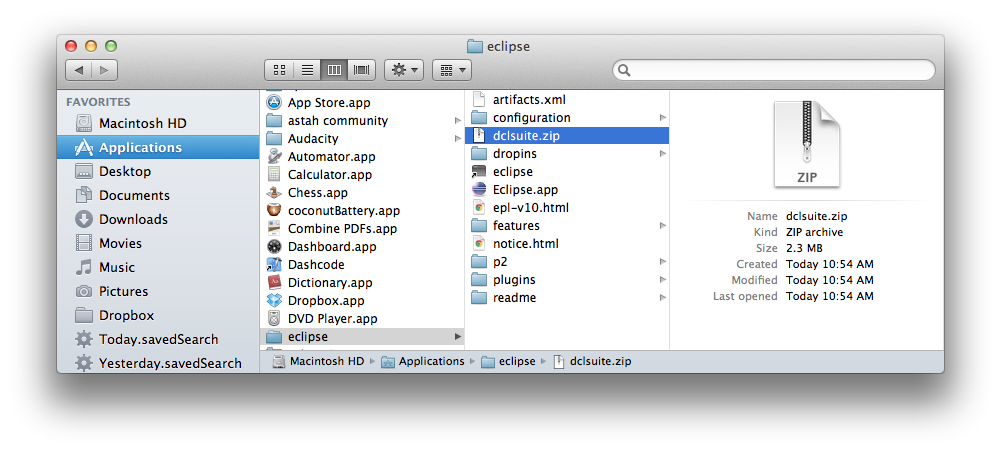
\includegraphics[width=12cm]{images/1.png}
	\end{block}
\end{frame}


\begin{frame}{\inserttitle}
	\begin{block}{\tiny After, check if the file $\tt dclsuite\_*.jar$ is inside directory $\tt eclipse/plugins$}
		\centering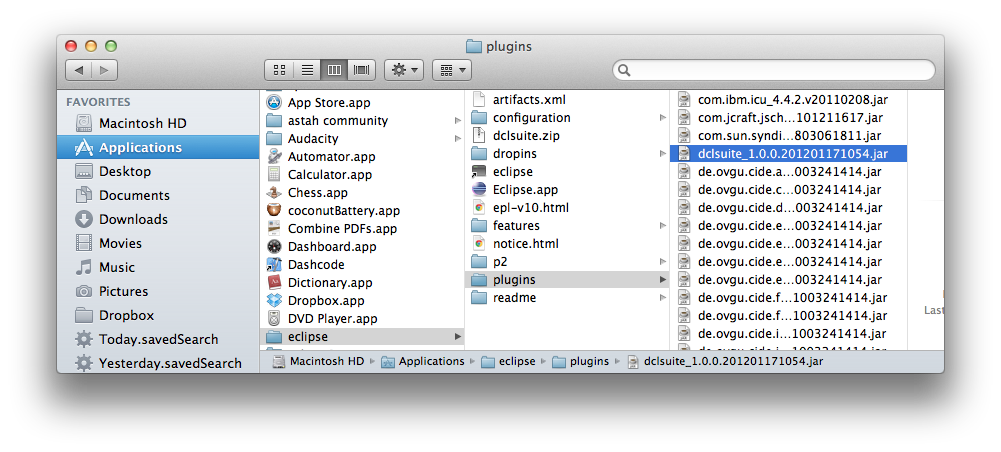
\includegraphics[width=12cm]{images/2.png}
	\end{block}
\end{frame}


\begin{frame}{\inserttitle}
	\begin{block}{\tiny Open Eclipse and, in the target Java Project, select $\tt Enable\; dclcheck$}
		\centering\includegraphics<1>[width=11.5cm]{images/3.png}
		\centering\includegraphics<2>[width=11.5cm]{images/3b.png}
	\end{block}
\end{frame}

\begin{frame}{\inserttitle}
	\begin{block}{\tiny A file $\tt architecture.dcl$ is created and opened}
		\centering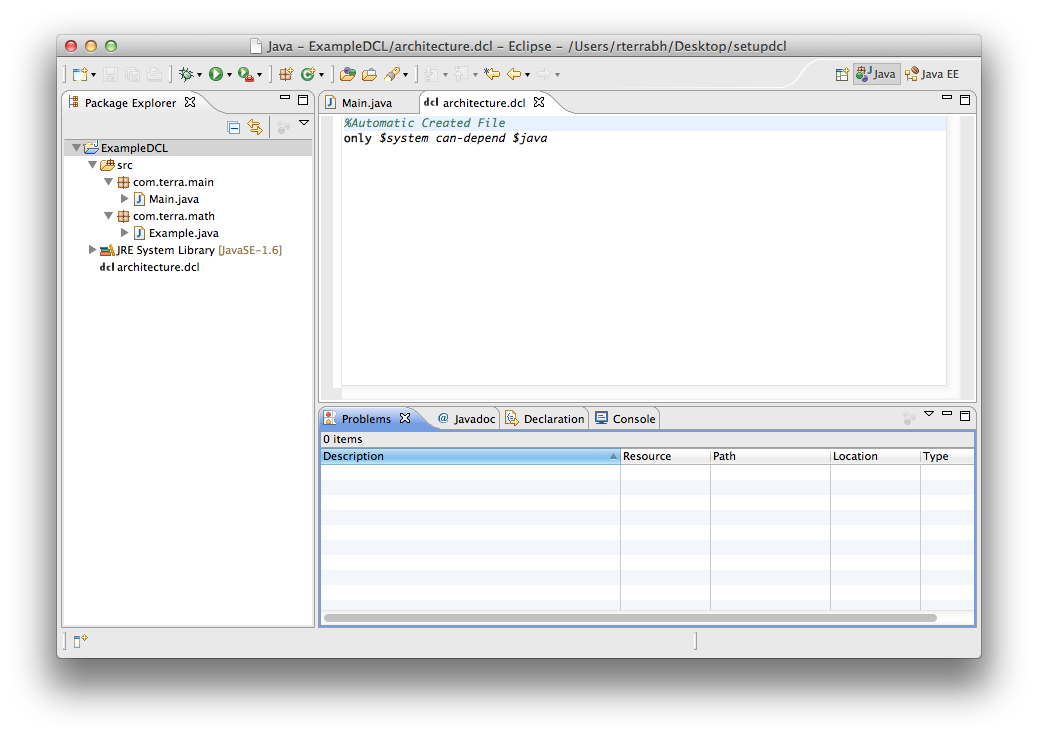
\includegraphics[width=11.5cm]{images/4.png}
	\end{block}
\end{frame}

\begin{frame}{\inserttitle}
	\begin{block}{\tiny For example, change the constraints and see the view $\tt Problems$}
		\centering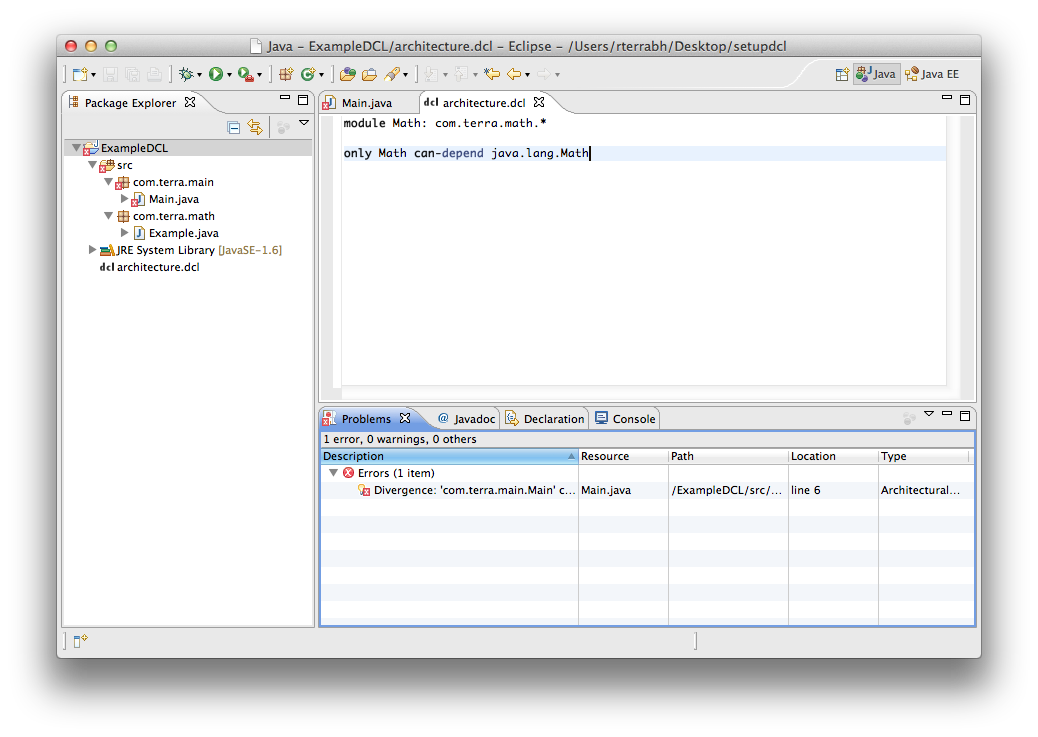
\includegraphics[width=11.5cm]{images/5.png}
	\end{block}
\end{frame}


\begin{frame}{\inserttitle}
	\begin{block}{\tiny Double click on an error goes to the location of the violation in the source code}
		\centering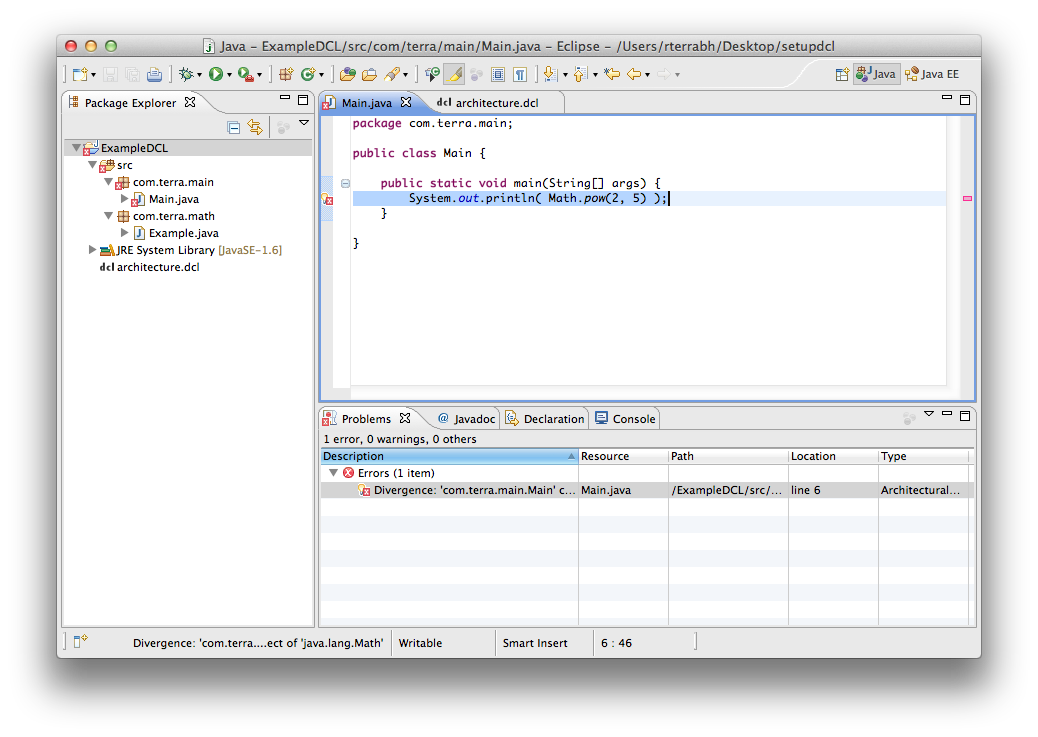
\includegraphics[width=11.5cm]{images/6.png}
	\end{block}
\end{frame}

\begin{frame}{\inserttitle}
	\begin{block}{\tiny You can access detailed informations about the violation}
		\centering\includegraphics<1>[width=11.5cm]{images/7.png}
		\centering\includegraphics<2>[width=10.9cm]{images/7b.png}
		\centering\includegraphics<3>[width=10.9cm]{images/7c.png}
	\end{block}
\end{frame}


\begin{frame}{\inserttitle}
	\begin{block}{\tiny As soon you save the file, new violations are detected (incremental building)}
		\centering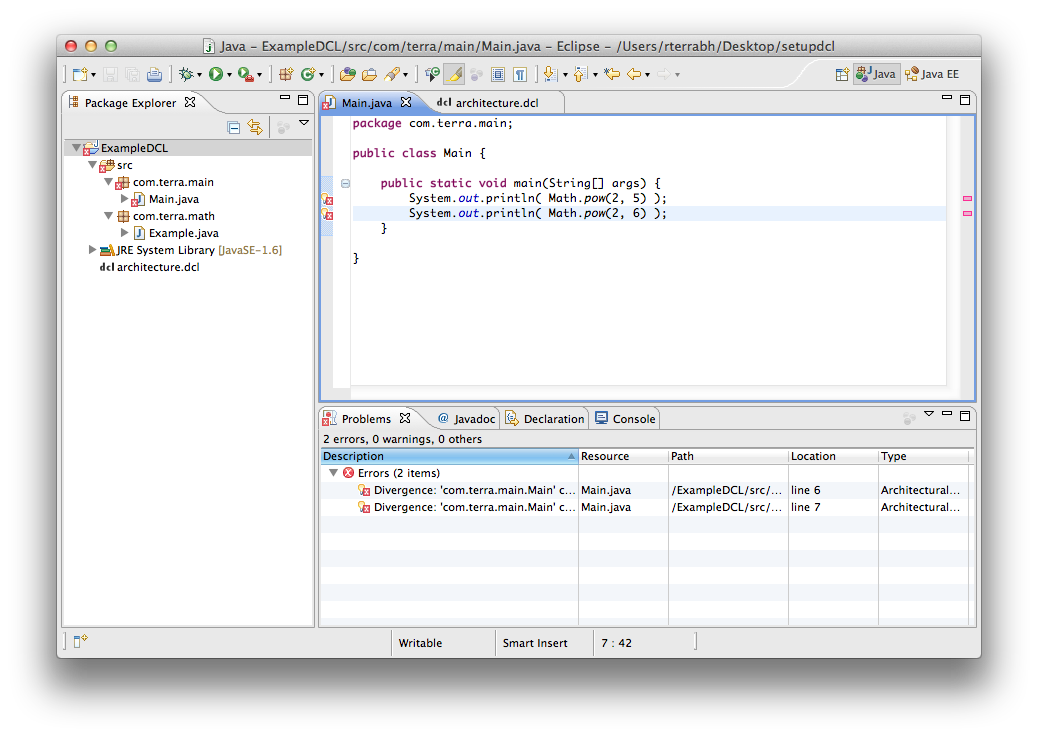
\includegraphics[width=11.5cm]{images/9.png}
	\end{block}
\end{frame}



\begin{frame}{\inserttitle}
	\begin{block}{\tiny Now, $\tt dclsuite$ is ready for use.\\~\\Moreover, a module to assist developers in fixing the detected violations is being developed.}
	\end{block}
\end{frame}

%
%
%
%
%
%
%
%
%




  


%\begin{frame}[t]
%	\begin{figure}
%		\includegraphics<1>[width=1cm]{a.jpeg}
%		\includegraphics<2>[width=1cm]{b.jpeg}
%	\end{figure}
%
%	\only<1>{\frametitle{Exemplo A}
%	
%	\begin{block}{Bloco A}
%		\begin{itemize}
%			\item Azinho
%			\item Azinho
%			\item Azinho
%		\end{itemize}
%	   \end{block}
%	
%	}
%	\only<2>{\frametitle{Exemplo B}
%	\begin{block}{Bloco B}
%		\begin{itemize}
%			\item Bezinho
%			\item Bezinho
%			\item Bezinho
%		\end{itemize}
%	   \end{block}
%	
%	
%	}	
%	
%
%\end{frame}


%\begin{frame}{}
%\begin{beamercolorbox}[center,shadow=false]{}
%\LARGE Perguntas???
%\end{beamercolorbox}
%\vspace{50pt}
%\begin{beamercolorbox}[center,shadow=false]{}
%\LARGE Obrigado!!!
%\end{beamercolorbox}
%\end{frame}

%\begin{frame}{}
%%\begin{figure}
%%     
\includegraphics[width=5cm]{int2.jpg}
%%\end{figure}
%%\vspace{50pt}
%\begin{beamercolorbox}[center,shadow=false]{}
%\Large Thanks!!!
%\end{beamercolorbox}
%
%\end{frame}


\end{document} %Insere agradecimento e fecha documento